% CS.tex
\chapter{Cubed-Sphere}

La Cubed-Sphere est constituée de six panels notés (I), ..., (VI) couvrant la sphère $\mathbb{S}_a^2$. Pour chacun de ces panels ils est possible d'associer des angles qui localisent un point ainsi que des bases covariantes et contravariantes qui permettent de calculer les opérateurs différentiels classiques.

\section{Localisation des points et bases $(\mathbf{g}_{\xi}, \mathbf{g}_{\eta})$}

Sur chaque panel on peut localiser un point grâce à un ensemble d'angles. De plus, une base de vecteur est donnée pour l'espace $\mathbb{T}\mathbb{S}_a^2$. Dans cette partie, on considère les points Nord : $N (0,0,a)$, Sud: $S (0,0,-a)$, Est: $E (0,a,0)$,Ouest: $W (0,-a,0)$, Front: $F(a,0,0)$ et Bottom: $B(-a,0,0)$. 

\subsection{Panel I}





\begin{figure}
\begin{center}
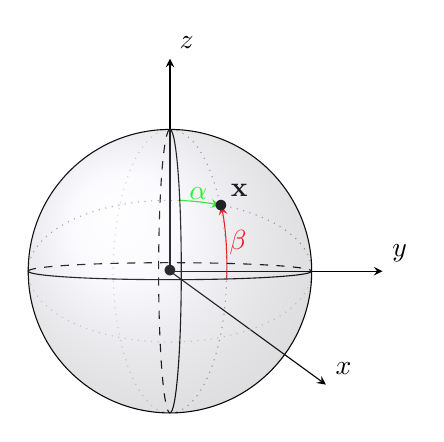
\begin{tikzpicture}[scale=1.8]
	\draw (0,0) node {$\bullet$} ;
	\draw [>=stealth, ->] (0,0) -- (1.5,0) ; 
	\draw (1.5,0) node[above right]{$y$} ;   
	\draw [>=stealth, ->] (0,0) -- (1.1,-0.8) ; 
	\draw (1.1,-0.8) node[above right]{$x$} ; 
	\draw [>=stealth, ->] (0,0) -- (0,1.5) ; 
	\draw (0,1.5) node[above right]{$z$} ; 

    \draw[>=stealth, ->,color=green] (0.065,0.5) arc (85:68:1cm and 0.5cm);
    \draw[color=green] (0.2,0.55) node{$\alpha$} ;
    \draw[>=stealth, ->,color=red] (0.4,-0.05) arc (-5:25:0.41cm and 1cm);
    \draw[color=red] (0.48,0.2) node{$\beta$} ;
    \draw (-1,0)[dotted, color=black!40] arc (180:360:1cm and -0.5cm);
    \draw (0,1)[dotted, color=black!40] arc (90:270:-0.4cm and 1cm);
    \draw (-1,0)[dotted, color=black!20] arc (180:360:1cm and 0.5cm);
    \draw (0,1)[dotted, color=black!20] arc (90:270:0.4cm and 1cm);
    
    \draw (-1,0) arc (180:360:1cm and 0.06cm);
    \draw (0,1) arc (90:270:-0.08cm and 1cm);
    \draw[dashed] (-1,0) arc (180:360:1cm and -0.06cm);
    \draw[dashed] (0,1) arc (90:270:0.08cm and 1cm);
    
    \draw (0.36,0.46) node {$\bullet$} ;
	\draw (0.36,0.46) node[above right]{$\mathbf{x}$} ;
    \draw (0,0) circle (1cm);
    \shade[ball color=blue!10!white,opacity=0.20] (0,0) circle (1cm);
\end{tikzpicture}
\hspace{1cm}
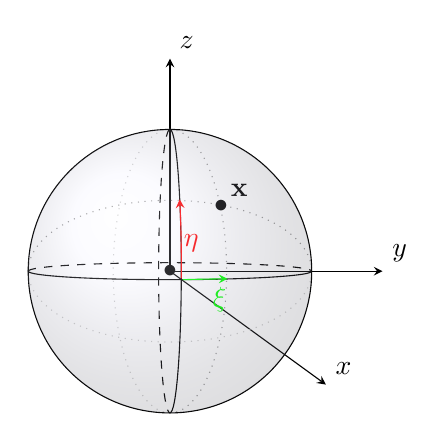
\begin{tikzpicture}[scale=1.8]
	\draw (0,0) node {$\bullet$} ;
	\draw [>=stealth, ->] (0,0) -- (1.5,0) ; 
	\draw (1.5,0) node[above right]{$y$} ;   
	\draw [>=stealth, ->] (0,0) -- (1.1,-0.8) ; 
	\draw (1.1,-0.8) node[above right]{$x$} ; 
	\draw [>=stealth, ->] (0,0) -- (0,1.5) ; 
	\draw (0,1.5) node[above right]{$z$} ; 
    
    \draw (-1,0)[dotted, color=black!40] arc (180:360:1cm and -0.5cm);
    \draw (0,1)[dotted, color=black!40] arc (90:270:-0.4cm and 1cm);
    \draw (-1,0)[dotted, color=black!20] arc (180:360:1cm and 0.5cm);
    \draw (0,1)[dotted, color=black!20] arc (90:270:0.4cm and 1cm);
    
    \draw (-1,0) arc (180:360:1cm and 0.06cm);
    \draw (0,1) arc (90:270:-0.08cm and 1cm);
    \draw[dashed] (-1,0) arc (180:360:1cm and -0.06cm);
    \draw[dashed] (0,1) arc (90:270:0.08cm and 1cm);
    
    \draw[>=stealth, ->,color=green] (0.09,-0.06) arc (225:247:1cm and -0.03cm);
    \draw[color=green] (0.35,-0.2) node{$\xi$} ;
    \draw[>=stealth, ->,color=red] (0.08,-0.05) arc (-5:28:0.1cm and 1cm);
    \draw[color=red] (0.15,0.2) node{$\eta$} ;
    
    \draw (0.36,0.46) node {$\bullet$} ;
	\draw (0.36,0.46) node[above right]{$\mathbf{x}$} ;
    \draw (0,0) circle (1cm);
    \shade[ball color=blue!10!white,opacity=0.20] (0,0) circle (1cm);
\end{tikzpicture}
\caption{Angles $(\alpha, \beta)$ (gauche) et $(\xi,\eta)$ (droite) associés au panel (I) de la Cubed-Sphere}
\label{alpha beta coord}
\end{center}
\end{figure}



Dans cette partie, on se concentre sur le panel $I$ pour le calcul.
Entre les différents systèmes de localisation, les relations suivantes sont vérifiées :

\begin{equation}
\left\lbrace
\begin{array}{rcccl}
x & = & a \cos \alpha \cos \eta & = & a \cos \beta \cos \xi \\
y & = & a \sin \alpha & = & a \cos \beta \sin \xi \\
z & = & a \cos \alpha \sin \eta & = & a \sin \beta \\
\end{array}
\right.
\end{equation}

On en déduit que :

\begin{equation}
\alpha = \arctan \left[ \dfrac{\tan \xi}{\sqrt{1 + \tan^2 \eta}} \right]
\end{equation}

ainsi que :

\begin{equation}
\beta = \arctan \left[ \dfrac{\tan \eta}{\sqrt{1 + \tan^2 \xi}} \right]
\end{equation}

et en dérivant :

\begin{equation}
\dfrac{\partial \alpha}{\partial \xi} = \cos \eta \dfrac{1+X^2}{1+\cos^2 \eta X^2} \hspace{1cm} \dfrac{\partial \beta}{\partial \eta} = \cos \xi \dfrac{1+Y^2}{1+\cos^2 \xi Y^2}
\end{equation}

La base locale $(\mathbf{g}_{\xi}, \mathbf{g}_{\eta})$ associée à $(\xi,\eta)$ est donnée par :

$$\mathbf{g}_{\xi} = \dfrac{\partial \mathbf{x}}{\partial \xi} \hspace{1cm} \mathbf{g}_{\eta} = \dfrac{\partial \mathbf{x}}{\partial \eta}.$$

Ainsi, en posant $\delta = \sqrt{1+X^2+Y^2}$, $\mathbf{g}_{\xi}$ et $\mathbf{g}_{\eta}$ sont donnés par :

\begin{equation}
\mathbf{g}_{\xi} = \dfrac{1+X^2}{\delta^2} \begin{pmatrix}
-y \\ x(1+Y^2) \\ -yY
\end{pmatrix} \text{ et } \mathbf{g}_{\eta} = \dfrac{1+Y^2}{\delta^2} \begin{pmatrix}
-z \\ -zX \\ x(1+X^2)
\end{pmatrix}
\label{base locale}
\end{equation}

\subsection{Tenseur métrique et base duale}

Pour tenir compte de la non-orthogonalité des coordonnées, il faut tenir compte de la métrique pour le calcul des opérateurs.

Le tenseur métrique est donné par :

\begin{equation}
\mathbf{G} = \begin{pmatrix}
\mathbf{g}_{\xi} \cdot \mathbf{g}_{\xi} & \mathbf{g}_{\xi} \cdot \mathbf{g}_{\eta} \\
\mathbf{g}_{\eta} \cdot \mathbf{g}_{\xi} & \mathbf{g}_{\eta} \cdot \mathbf{g}_{\eta}
\end{pmatrix}
\end{equation}

Ainsi, après calcul, on a :

\begin{equation}
\mathbf{G} = \begin{pmatrix}
G_{1,1} & G_{1,2} \\ G_{2,1} & G_{2,2}
\end{pmatrix} = a^2 \dfrac{(1+X^2)(1+Y^2)}{\delta^4} \begin{pmatrix}
1+X^2 & -XY \\ -XY & 1+Y^2
\end{pmatrix}
\end{equation}

que l'on peut inverser en :

\begin{equation}
\mathbf{G}^{-1} = \begin{pmatrix}
G^{1,1} & G^{1,2} \\ G^{2,1} & G^{2,2}
\end{pmatrix} = \dfrac{\delta^2}{a^2 (1+X^2)(1+Y^2)} \begin{pmatrix}
1+Y^2 & XY \\ XY & 1+X^2
\end{pmatrix}
\end{equation}

Il est important de connaitre la base duale par rapport à la métrique $\mathbf{G}$. On cherche $\mathbf{g}_{\xi}$ et $\mathbf{g}_{\eta}$ tels que :

\begin{equation}
\left\lbrace
\begin{array}{rcccl}
\mathbf{g}_{\xi} \cdot \mathbf{g}^{\xi} & = & \mathbf{g}_{\eta} \cdot \mathbf{g}^{\eta} & = & 1 \\
\mathbf{g}_{\xi} \cdot \mathbf{g}^{\eta} & = & \mathbf{g}_{\eta} \cdot \mathbf{g}^{\xi} & = & 0 \\
\end{array}
\right.
\end{equation}

d'où la relation suivante :

\begin{equation}
\left\lbrace
\begin{array}{rcl}
\mathbf{g}^{\xi} & = & G^{1,1} \mathbf{g}_{\xi} + G^{1,2} \mathbf{g}_{eta} \\
\mathbf{g}^{\eta} & = & G^{2,1} \mathbf{g}_{\xi} + G^{2,2} \mathbf{g}_{eta} \\
\end{array}
\right.
\end{equation}

d'où :

\begin{equation}
\mathbf{g}^{\xi} = \dfrac{1}{x(1+X^2)}\begin{pmatrix}
-X \\ 1 \\ 0
\end{pmatrix} \text{ et } \mathbf{g}^{\eta} = \dfrac{1}{x(1+Y^2)}\begin{pmatrix}
-Y \\ 0 \\ 1
\end{pmatrix}
\end{equation}

$( \mathbf{g}^{\xi}, \mathbf{g}^{\eta})$ est la base duale de $(\mathbf{g}_{\xi}, \mathbf{g}_{\eta})$ par rapport à la métrique $\mathbf{G}$.

\subsection{Symboles de Christophel}

Les champs de vecteur $( \mathbf{g}^{\xi}, \mathbf{g}^{\eta})$ et $( \mathbf{g}_ {\xi}, \mathbf{g}_{\eta})$ sont tangents à la sphère. En conséquence, ils varient (continuement) en fonction de $\xi$ et $\eta$. On définit les symboles de Christoffel par :

\begin{equation}
\left\lbrace
\begin{array}{rcl}
\dfrac{\partial \mathbf{g}_{\xi}}{\partial \xi} & = & \Gamma_{\xi,\xi}^{\xi} \mathbf{g}_{\xi} + \Gamma_{\xi,\xi}^{\eta} \mathbf{g}_{\eta}\\

\dfrac{\partial \mathbf{g}_{\xi}}{\partial \eta} & = & \Gamma_{\eta,\xi}^{\xi} \mathbf{g}_{\xi} + \Gamma_{\eta,\xi}^{\eta} \mathbf{g}_{\eta}\\

\dfrac{\partial \mathbf{g}_{\eta}}{\partial \xi} & = & \Gamma_{\xi,\eta}^{\xi} \mathbf{g}_{\xi} + \Gamma_{\xi,\eta}^{\eta} \mathbf{g}_{\eta}\\

\dfrac{\partial \mathbf{g}_{\eta}}{\partial \eta} & = & \Gamma_{\eta,\eta}^{\xi} \mathbf{g}_{\xi} + \Gamma_{\eta,\eta}^{\eta} \mathbf{g}_{\eta}\\
\end{array}
\right.
\end{equation}

\begin{remarque}
On note que $\Gamma_{\eta,\xi}^{\xi}=\Gamma_{\xi,\eta}^{\xi}$ et $\Gamma_{\eta,\xi}^{\eta}=\Gamma_{\xi,\eta}^{\eta}$.

En effet :

$$\Gamma_{\xi, \eta}^{\eta} = \left( \dfrac{\partial \mathbf{g}_{\eta}}{\partial \xi} \right) \cdot \mathbf{g}^{\eta} = \left( \dfrac{\partial}{\partial \xi} \dfrac{\partial \mathbf{x}}{\partial \eta} \right) \cdot \mathbf{g}^{\eta} = \left( \dfrac{\partial}{\partial \eta} \dfrac{\partial \mathbf{x}}{\partial \xi} \right) \cdot \mathbf{g}^{\eta} = \left( \dfrac{\partial \mathbf{g}_{\xi}}{\partial \eta} \right) \cdot \mathbf{g}^{\eta} = \Gamma_{\eta, \xi}^{\eta}$$

de même pour $\Gamma_{\eta,\xi}^{\xi}=\Gamma_{\xi,\eta}^{\xi}$.
\end{remarque}

\begin{proposition}
Les relations suivantes sont vérifiées :

\begin{equation}
\left\lbrace
\begin{array}{rcccl}
\Gamma_{\xi,\xi}^{\xi} & = & \left[ \dfrac{\partial \mathbf{g}_{\xi}}{\partial \xi} \right] \cdot \mathbf{g}^{\xi} & = & - \left[ \dfrac{\partial \mathbf{g}^{\xi}}{\partial \xi} \right] \cdot \mathbf{g}_ {\xi}\\

\Gamma_{\xi,\xi}^{\eta} & = & \left[ \dfrac{\partial \mathbf{g}_{\xi}}{\partial \xi} \right] \cdot \mathbf{g}^{\eta} & = & - \left[ \dfrac{\partial \mathbf{g}^{\eta}}{\partial \xi} \right] \cdot \mathbf{g}_ {\xi}\\

\Gamma_{\xi,\eta}^{\xi} & = & \left[ \dfrac{\partial \mathbf{g}_{\eta}}{\partial \xi} \right] \cdot \mathbf{g}^{\xi} & = & - \left[ \dfrac{\partial \mathbf{g}^{\xi}}{\partial \xi} \right] \cdot \mathbf{g}_ {\eta}\\

\Gamma_{\xi,\eta}^{\eta} & = & \left[ \dfrac{\partial \mathbf{g}_{\eta}}{\partial \xi} \right] \cdot \mathbf{g}^{\eta} & = & - \left[ \dfrac{\partial \mathbf{g}^{\eta}}{\partial \xi} \right] \cdot \mathbf{g}_ {\eta}\\

\Gamma_{\eta,\eta}^{\eta} & = & \left[ \dfrac{\partial \mathbf{g}_{\eta}}{\partial \eta} \right] \cdot \mathbf{g}^{\eta} & = & - \left[ \dfrac{\partial \mathbf{g}^{\eta}}{\partial \eta} \right] \cdot \mathbf{g}_ {\eta}\\

\Gamma_{\eta,\eta}^{\xi} & = & \left[ \dfrac{\partial \mathbf{g}_{\eta}}{\partial \eta} \right] \cdot \mathbf{g}^{\xi} & = & - \left[ \dfrac{\partial \mathbf{g}^{\xi}}{\partial \eta} \right] \cdot \mathbf{g}_ {\eta}\\
\end{array}
\right.
\end{equation}
\end{proposition}

\begin{proof}
Nous ne démontrons que la première équalité, les autres égualités se retrouvent de manière extrêmement similaire.

$$\left[ \dfrac{\partial \mathbf{g}_{\xi}}{\partial \xi} \right] \cdot \mathbf{g}^{\xi} = \left[ \Gamma_{\xi,\xi}^{\xi} \mathbf{g}_{\xi} + \Gamma_{\xi,\xi}^{\eta} \mathbf{g}_{\eta} \right] \cdot \mathbf{g}^{\xi}$$

Or $\mathbf{g}_{\xi} \cdot \mathbf{g}^{\eta} = 1$ et $\mathbf{g}_{\eta} \cdot \mathbf{g}^{\eta} = 0$, d'où la première partie :

$$\Gamma_{\xi,\xi}^{\xi} = \left[ \dfrac{\partial \mathbf{g}_{\xi}}{\partial \xi} \right] \cdot \mathbf{g}^{\xi}.$$

D'autres part, on a :

$$\Gamma_{\xi,\xi}^{\xi} = \left[ \dfrac{\partial \mathbf{g}_{\xi}}{\partial \xi} \right] \cdot \mathbf{g}^{\xi} = \dfrac{\partial}{\partial \xi}  \underbrace{\left(\mathbf{g}_{\xi} \cdot \mathbf{g}^{\xi}\right)}_{=1}  - \left[ \dfrac{\partial \mathbf{g}^{\xi}}{\partial \xi}  \right] \cdot \mathbf{g}_{\xi} = - \left[ \dfrac{\partial \mathbf{g}^{\xi}}{\partial \xi}  \right] \cdot \mathbf{g}_{\xi}$$

et la relation est démontrée.
\end{proof}

On peut calculer les dérivées suivantes :

\begin{equation}
\dfrac{\partial \mathbf{g}^{\xi}}{\partial \xi} = \dfrac{1}{x} \begin{pmatrix}
-\dfrac{X^2}{\delta^2}+2X \cos \xi \sin \xi -1 \\ \dfrac{X}{\delta^2}-2 \cos \xi \sin \xi \\ 0
\end{pmatrix}
\text{ et }
\dfrac{\partial \mathbf{g}^{\xi}}{\partial \eta} = \dfrac{1+Y^2}{\delta^2 x^2 (1+X^2)} \begin{pmatrix}
-X \\ 1 \\ 0
\end{pmatrix}
\end{equation}

de même :

\begin{equation}
\dfrac{\partial \mathbf{g}^{\eta}}{\partial \xi} = \dfrac{X(1+X^2)}{x \delta^2 (1+Y^2)} \begin{pmatrix}
-Y \\ 0 \\ 1
\end{pmatrix}
\text{ et }
\dfrac{\partial \mathbf{g}^{\eta}}{\partial \eta} = \dfrac{1}{x} \begin{pmatrix}
- \dfrac{Y^2}{\delta^2} + 2 Y \cos \eta \sin \eta -1 \\ 0 \\ \dfrac{Y}{\delta^2}- 2 \cos \eta \sin \eta
\end{pmatrix}
\end{equation}

d'où les symboles de Christoffel :

\begin{equation}
\left\lbrace
\begin{array}{rcl}
\Gamma_{\xi,\eta}^{\xi} & = & - \dfrac{Y ( 1+Y^2)}{\delta^2}\\
\Gamma_{\xi,\eta}^{\eta} & = & - \dfrac{X(1+X^2)}{\delta^2}\\
\Gamma_{\eta,\eta}^{\xi} & = & 0 \\
\Gamma_{\xi,\xi}^{\eta} & = & 0 \\
\Gamma_{\eta,\eta}^{\eta} & = & \dfrac{1+Y^2}{\delta^2} \left[ 2 \delta^2 \cos \eta \sin \eta - Y \right]\\
\Gamma_{\xi,\xi}^{\xi} & = & \dfrac{1+X^2}{\delta^2} \left[ 2 \delta^2 \cos \xi \sin \xi - X \right]
\end{array}
\right.
\end{equation}

\begin{proposition}
Les symboles de Christoffel sont invariants par changement de face
\end{proposition}

\begin{proof}
Soit $R_f$ la rotation permettant de passer d'une face à une autre. On note en particulier que $R_f$ est indépendant de $\xi$ et $\eta$.

Alors soit $K$ et $L$ dans $\left\lbrace I, II, III, IV, V, VI \right\rbrace$ et $\tau$, $\upsilon \in \left\lbrace \xi, \eta \right\rbrace$. Alors par propriété du produit scalaire :

$$\left( \dfrac{\partial}{\partial \tau}  R_f \mathbf{g}_{\tau} \right) \cdot \left( R_f \mathbf{g}_{\upsilon} \right) = \left( R_f \dfrac{\partial}{\partial \tau}   \mathbf{g}_{\tau} \right) \cdot \left( R_f \mathbf{g}_{\upsilon} \right) =  \left( \dfrac{\partial}{\partial \tau}  \mathbf{g}_{\tau} \right) \cdot \left( R_f^{-1} R_f \mathbf{g}_{\upsilon} \right) =  \left( \dfrac{\partial}{\partial \tau}  \mathbf{g}_{\tau} \right) \cdot \left( \mathbf{g}_{\upsilon} \right)$$

de même :

$$\left( \dfrac{\partial}{\partial \upsilon}  R_f \mathbf{g}_{\tau} \right) \cdot \left( R_f \mathbf{g}_{\upsilon} \right) =  \left( \dfrac{\partial}{\partial \upsilon} \mathbf{g}_{\tau} \right) \cdot \left( \mathbf{g}_{\upsilon} \right)$$

et on retrouve l'ensemble des symboles de Christoffel.
\end{proof}































